% Diese Zeile bitte -nicht- aendern.
\documentclass[course=erap]{aspdoc}
%%%%%%%%%%%%%%%%%%%%%%%%%%%%%%%%%
\graphicspath{ {./images/} }
\usepackage[font=small,labelfont=bf]{caption}
%%%%%%%%%%%%%%%%%%%%%%%%%%%%%%%%%
%% TODO: Ersetzen Sie in den folgenden Zeilen die entsprechenden -Texte-
%% mit den richtigen Werten.
\newcommand{\theGroup}{142} % Beispiel: 42
\newcommand{\theNumber}{A213} % Beispiel: A123
\author{Anton Baumann \and Felix Brandis \and Michal Cizevskij}
\date{Sommersemester 2020} % Beispiel: Wintersemester 2019/20
%%%%%%%%%%%%%%%%%%%%%%%%%%%%%%%%%

% Diese Zeile bitte -nicht- aendern.
\title{Gruppe \theGroup{} -- Abgabe zu Aufgabe \theNumber}

\usepackage{subfig}

\begin{document}
\maketitle

\section{Einleitung}

Um die in der Vorlesung erlangten Kenntnisse zu vertiefen, wird vom Lehrstuhl für Rechnerarchitektur und Parallele Systeme ein Semester begleitendes Praktikum angeboten.\\
Im Rahmen dieses Rechnerarchitektur Praktikums hat sich unsere Gruppe mit dem Thema der Moore Kurve auseinandergesetzt. Die Moore Kurve ist eine von dem Mathematiker Eliakim Hastings Moore (1862-1932) entwickelte raumfüllende Kurve. Sie basiert auf der Hilbert Kurve und findet oft Anwendung in Bildverarbeitung und Datendarstellung. Unsere erste Aufgabe war es einen Algorithmus in Assembler zu entwickeln, der die Moore Kurve beliebigen Grades erstellt und in einer Datei abbildet. Die zweite Aufgabe war es zu beantworten, ob es möglich ist einen beliebigen Punkt der Kurve in konstanter Zeit unabhängig vom Grad zu berechnen.\\
\\
\begin{center}
    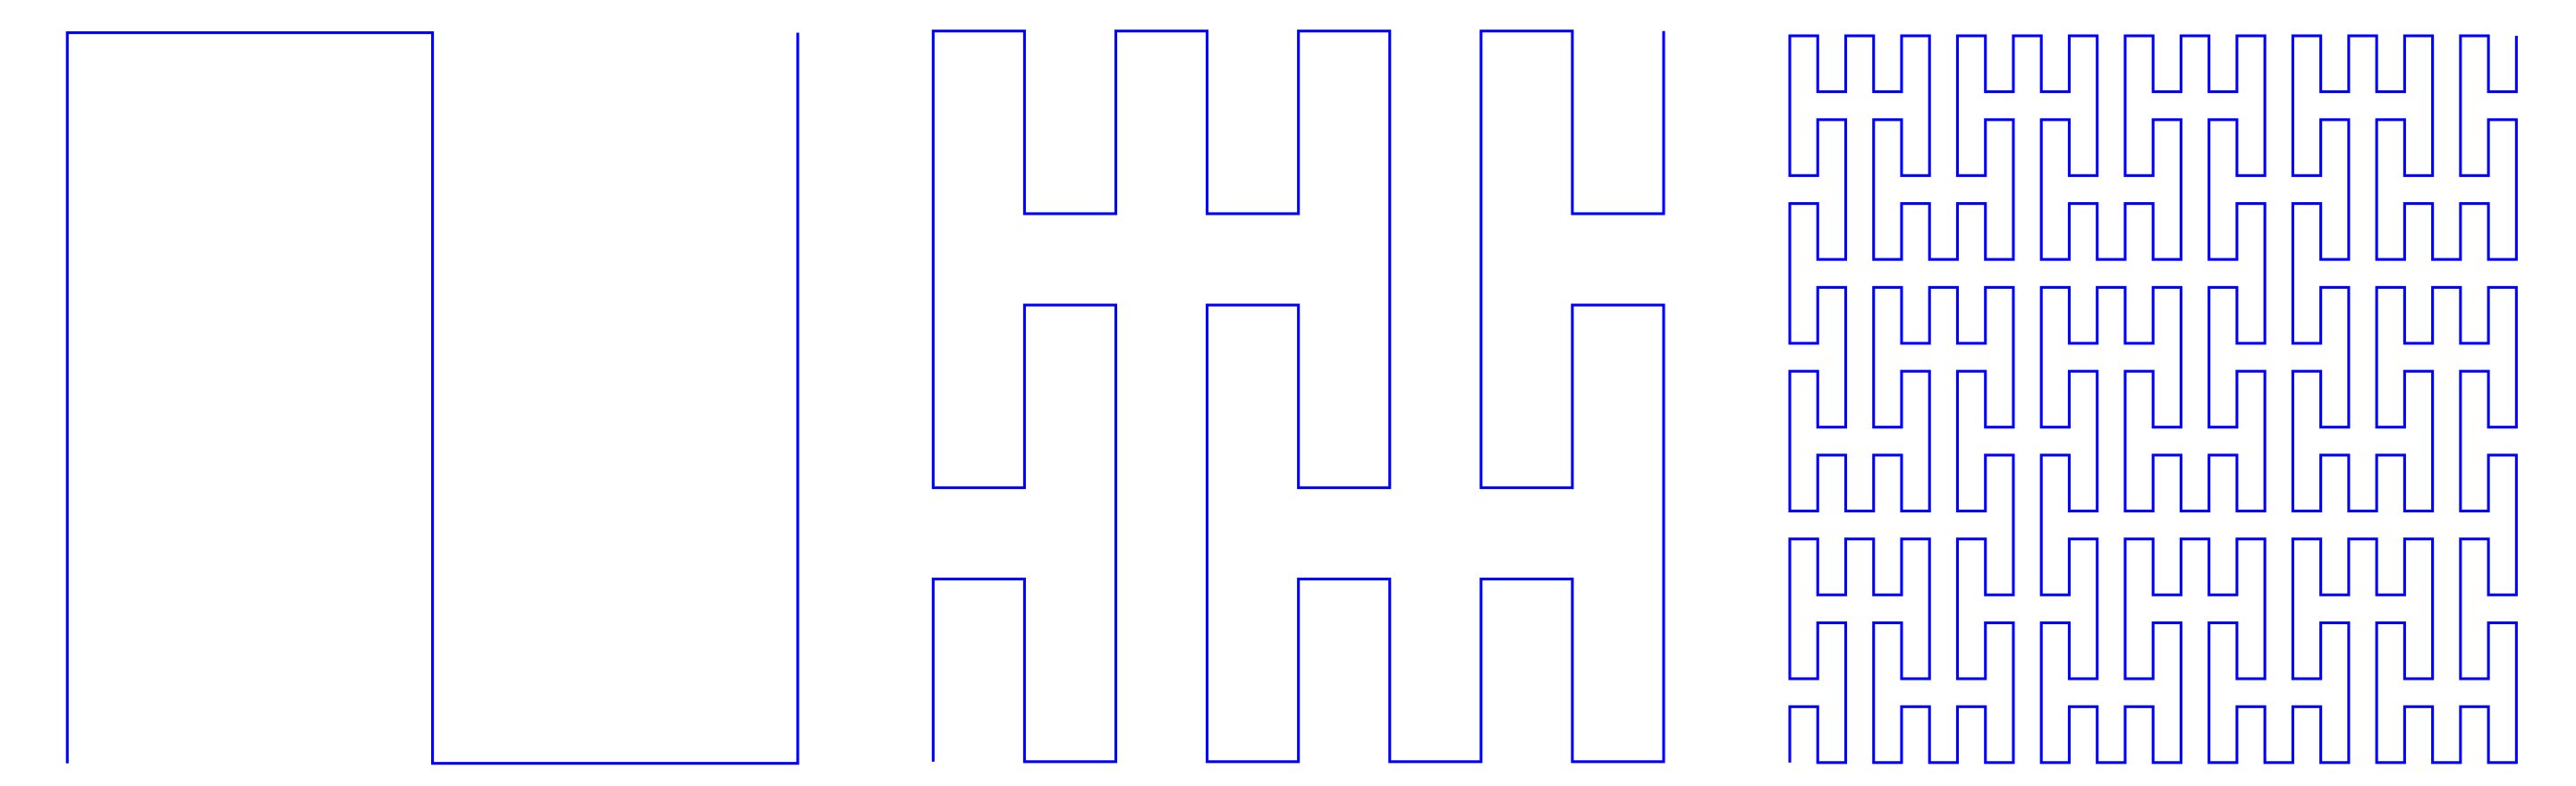
\includegraphics[width=12cm, height=4cm]{Peano}\\ %cite
    \tiny Figur 1: Die drei ersten Iterationen der Peano Kurve
\end{center}
\   \\
Generell ist eine raumfüllenden Kurve (Englisch: space-filling curve oder auch SFC) eine "Linie" die von einem Eindimensionalen Raum auf ein N-Dimensionalen Raum abbildet. Einfachheitshalber beschränken wir uns aber auf zweidimensionalen und ein Beispiel im dreidimensionalen Raum. Die Besonderheit dieser Kurve liegt darin, dass sie jeden Punkt des Einheitsquadrats passiert. Genauer gesagt, wenn n für den Grad der Kurve steht und $\lim_{n\to\infty}$, dann wird eine gegebene Fläche durch so eine Kurve gefüllt.\\
Die erste SFC wurde von einem Italienischen Mathematiker Giuseppe Peano in 1890 entwickelt. 
\newpage
Die Motivation für solch eine Erkenntnis bekam er durch einen weitern  renommierten Mathematiker Georg Cantor der wenige Jahre zuvor bewiesen hatte, dass die \\ Mengen der Natürlichen zahlen und die der positiven rationalen Zahlen gleich mächtig sind (Cantors erstes diagonal Argument). 
Durch das verallgemeinern des Cantorischen Diagonalarguments kann man zeigen, dass es eindimensionale Objekte gibt, \\ die zweidimensionale füllen können. Eine raumfüllende Kurve ist also eine surjektive Abbildung, die von einem Einheitsintervall in ein Einheitsquadrat abbildet.
\\
\\
\begin{center}
    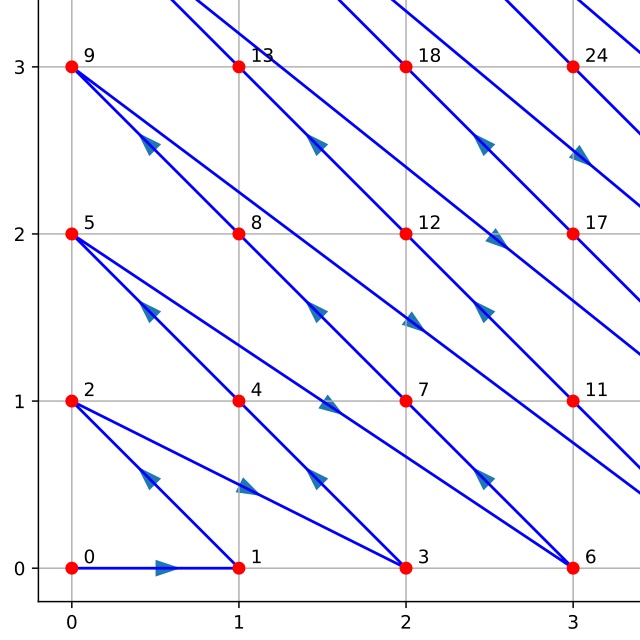
\includegraphics[width=5cm, height=5cm]{Cantor}\\   %cite
    \tiny Figur 2: Cantorische Paarungsfunktion
\end{center}
\   \\
\\
Die Hilbert Kurve, die von dem gleichnamigen Mathematiker David Hilbert in 1891 entwickelt wurde ist eine einfachere Version die das Einheitsquadrat in 4 Teile anstatt 9 partitioniert. Diese Quadranten beinhalten dann die Hilbert Kurve vom Grad n - 1. Betrachtet man zum Beispiel die mittlere Abbildung in Fig. 3 ,entsprechend Hilbert von Grad 2. Dann bemerkt man, dass sie vier mal die Kurve vom Grad 1 beinhaltet, die rotiert oder gespiegelt wurde und an den End- bzw. Startpunkten verbunden wurden.
\\
\\
\begin{center}
    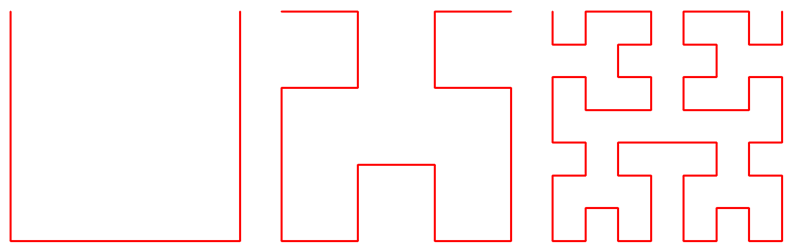
\includegraphics[width=12cm, height=4cm]{Hilbert}\\ %cite
    \tiny Figur 3: Die drei ersten Iterationen der Hilbert Kurve
\end{center}
\   \\
\newpage %Autor der Moore Kurve ist im Abstract erwähnt fehlt datum leider
Wie bereits erwähnt ist die Moore Kurve eine Variation der Hilbert Kurve. Die ersten Grade der Moore- und Hilbert-Kurve sind äquivalent. Dabei ergeben sich die weiteren Iterationen der Moore Kurve, durch die Zusammensetzung der Hilbert Kurve vom Grad n - 1.  Also bis zum Grad n -1 zeichnet man eine Hilbert Kurve, jedoch beim Grad n ordnet man die 4 Hilbert Kurven vom Grad n - 1 anders an.\\ % wie genau ist dann Lösungsweg
Bemerkenswert ist, dass im Gegensatz zur Hilbert Kurve, die Moore Kurve so konstruiert ist, sodass der Anfangspunkt und Endpunkt sich nebeneinander befinden.
\\
\\
\begin{center}
    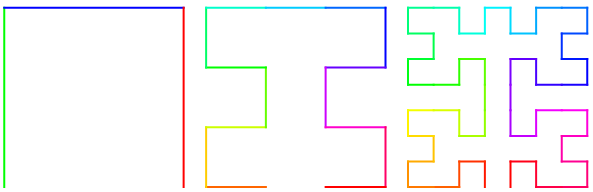
\includegraphics[width=12cm, height=4cm]{Moore}\\   %cite
    \tiny Figur 4: Die drei ersten Iterationen der Moore Kurve
\end{center}
\   \\
Außerdem gehört die Moore Kurve (Peano und Hilbert ebenfalls) einer Unterkategorie der SFC die man FASS Kurven nennt. (FASS: „space-filling, self-avoiding, simple and self-similar“).\\
Dies birgt wichtige Eigenschaften weshalb sie in der Praxis Verwendung findet. Zu einem die Kurve ist selbst ausweichend, das bedeutet jeder Punkt ist exakt festgelegt, also wird er nur einmal durchlaufen. Hinzu behält die Kurve die Lokalität der Punkte bei. Das bedeutet, sind die Punkte nah beinander im eindimensionalen Einheitsintervall, so sind sie es ebenfalls in der Kurve. % http://blog.christianperone.com/2015/08/googles-s2-geometry-on-the-sphere-cells-and-hilbert-curve/
\\
\\
\begin{center}
    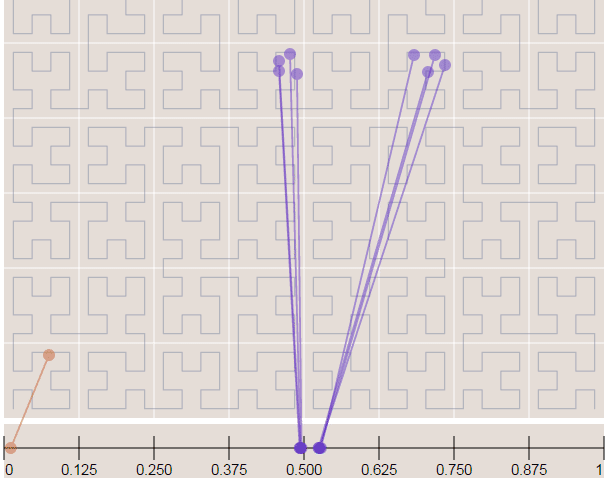
\includegraphics[width=8cm, height=6cm]{Locality}\\ %cite
    \tiny Figur 5: Graphik um die Eigenschaft der Lokalität zu verdeutlichen % for spatial DB = raumbezogene Datenbank
\end{center} 
\newpage 

In raumbezogenen Anwendungen kommt es oft vor, dass raumfüllende Kurven verwendet werden, um effizient geographische Daten die in eindimensionaler oder zweidimensionaler Form vorhanden sind in eindimensionale Daten umzuwandeln. \\Dafür teilt man  sein Gebiet in Zellen auf. Diese dienen dann einer kompakten \\ Darstellung der bestimmten Region. Um diese Zellen schnell "`ansprechen"' zu können indexieren wir sie. Dabei ist es uns wichtig, dass sie Sinnvoll indexiert werden, sodass geographisch naheliegende Zellen, es ebenso es im Feld tun.
Da eine FASS Kurve genau diese Anforderungen erfüllt eignet sie sich besonders gut für solch eine Verwendung. Ein konkretes Beispiel der Anwendung wäre die \href{https://code.google.com/archive/p/s2-geometry-library/}{S2-geometry-library von Google}. 

% vielleicht noch erwähnen das es alternativen gibt aber zb Hilbert kurve sehr effizient ist
\begin{figure}
    \centering
    \begin{minipage}{0.45\textwidth}
        \centering
        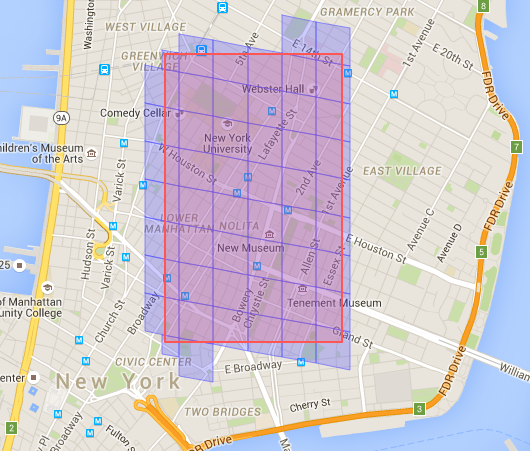
\includegraphics[width=0.9\textwidth]{Map}\\
        \tiny Figur 6: Einteilung von New York in Zellen
    \end{minipage}\hfill
    \begin{minipage}{0.45\textwidth}
        \centering
        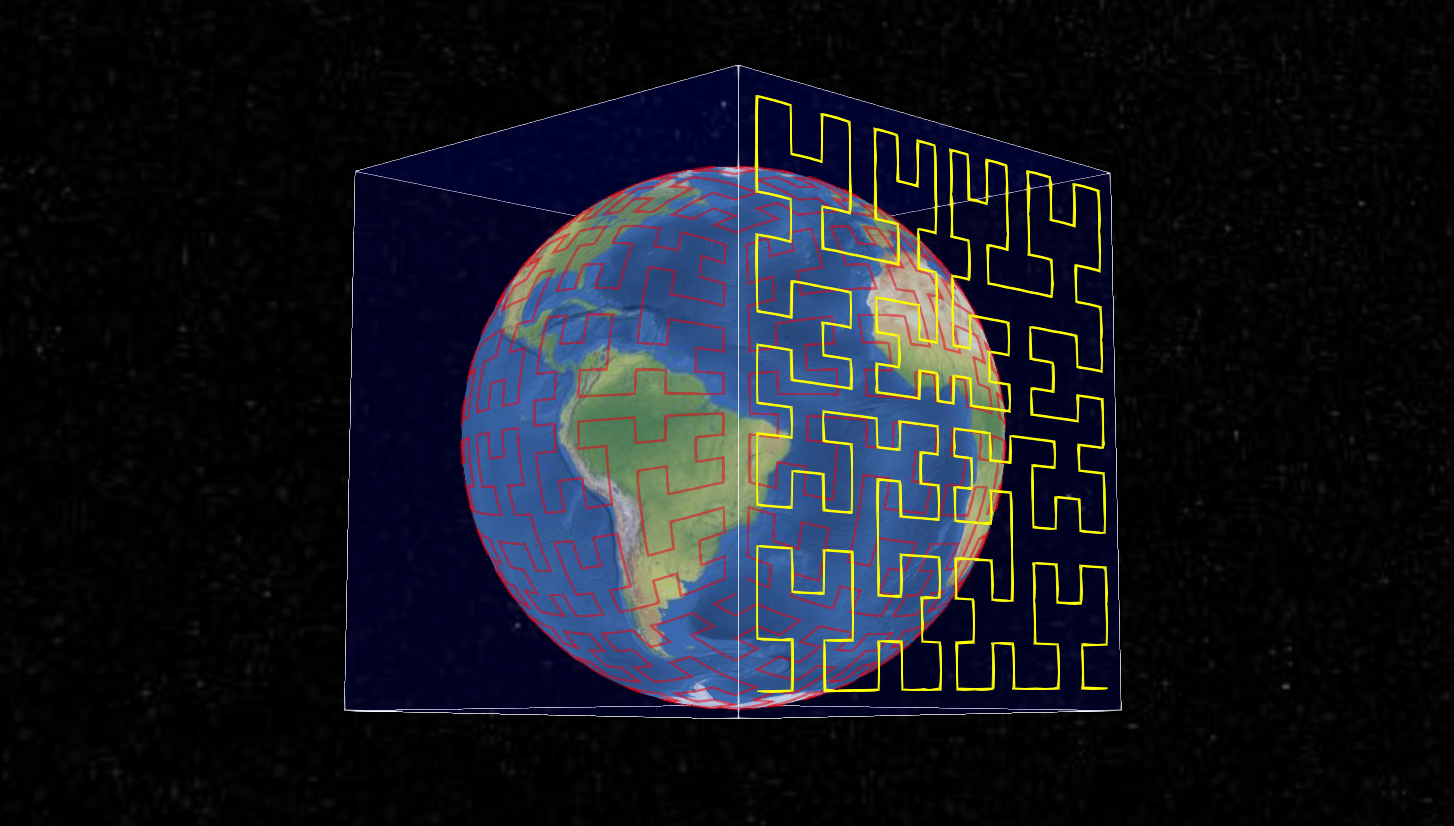
\includegraphics[width=0.9\textwidth]{Earth} \\
        \tiny Figur 7: Hilbert projeziert auf die Erde
    \end{minipage}
\end{figure}

%https://medium.com/sidewalk-talk/s2-cells-and-space-filling-curves-keys-to-building-better-digital-map-tools-for-cities-a312aa5e2f59


%\begin{center}
%   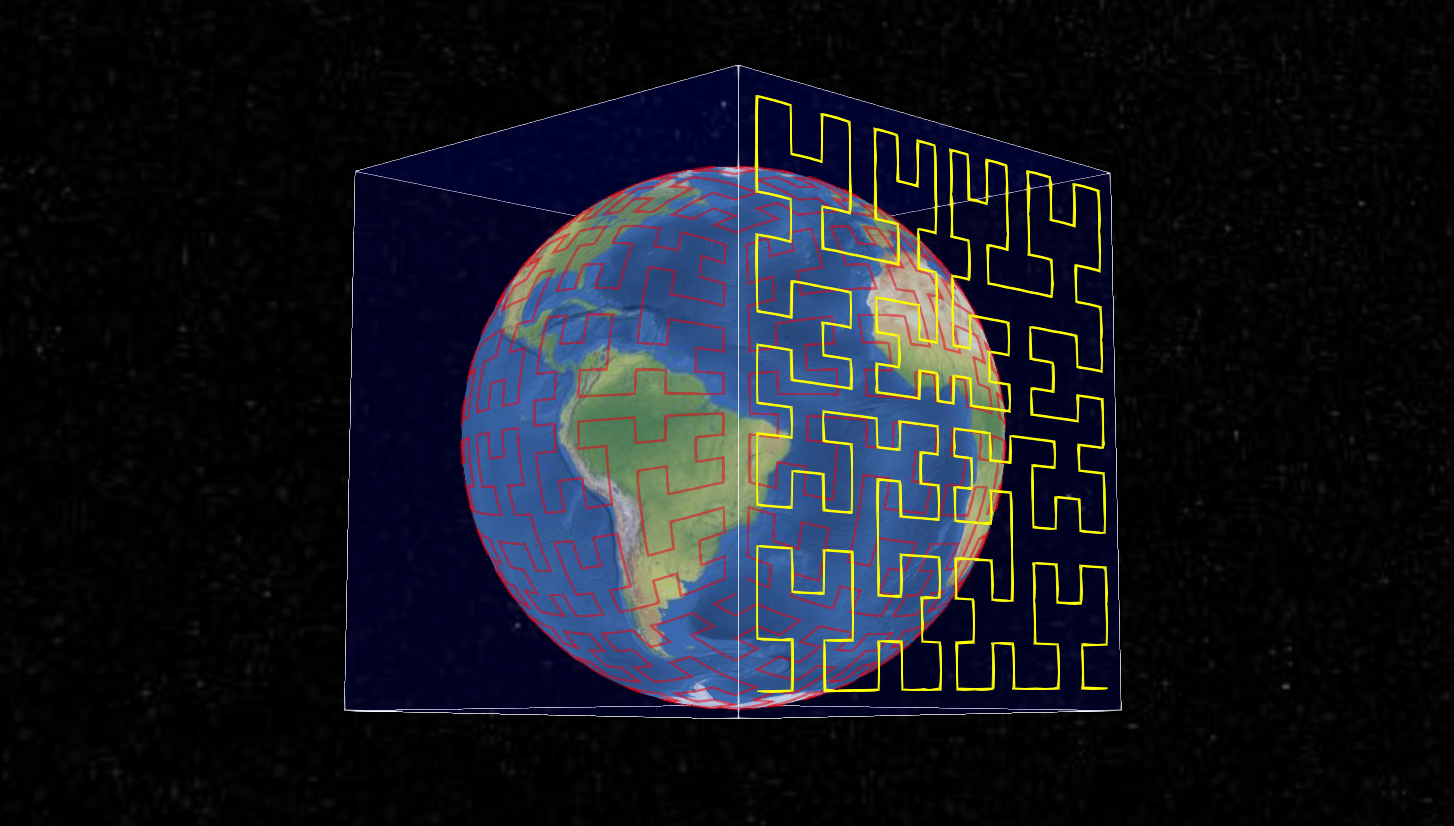
\includegraphics[width=9cm, height=6cm]{Earth}\\    %cite
%   \tiny Abbildung 6: Einteinlung der Erde 
%\end{center}


\section{Lösungsansatz}


% TODO: Je nach Aufgabenstellung einen der Begriffe wählen
\section{Korrektheit/Genauigkeit}


\section{Performanzanalyse}
Um das Laufzeitzeitverhalten unserer Implementierung der Moore-Kurve zu überprüfen und beurteilen, haben wir Benchmarks folgender vier Implementierungen auf einem MaxBook Pro mit einem 3,1 Ghz Dual-Core Intel i7 und 16 Gb 1867 Mhz DDR3 RAM durchgeführt.

\begin{center}
    \begin{tabular}{| r | r | r | r | r | r | r |}
    \hline
    Grad \textit{n} & \# Punkte & Speicher & \textit{asm\_avx} & \textit{asm} & \textit{c\_batch} & \textit{c\_iter}  \\ \hline
    3 & 64 & 512 B  & 27 ns & 23 ns & 67 ns & 1796 ns \\  \hline
    6 & 4096 & 32 KiB  & 601 ns & 1213 ns & 6524 ns & 219 $\mu s$ \\  \hline
    9 & 26144 & 2048 KiB  & 179 $\mu s$ & 289 $\mu s$ & 830 $\mu s$ & 16562 $\mu s$  \\  \hline
    12 & 16,78 * 1e6 & 128 MiB & 21,5 ms & 24,5 ms & 94,3 ms & 1303,1 ms \\ \hline
    15 & 1,07 * 1e9 & 8 GiB & 1575,9 ms & 1607,4 ms & 7108,1 ms & 92985,2 ms \\ \hline
    16 & 4,29 * 1e9 & 32 GiB & 108,3 s & 125,7 s & 175,9 s & 718,1 s \\ \hline
    \end{tabular}
\end{center}

\begin{figure}[htbp] 
    \centering
    \subfloat[alle Implementierungen]{{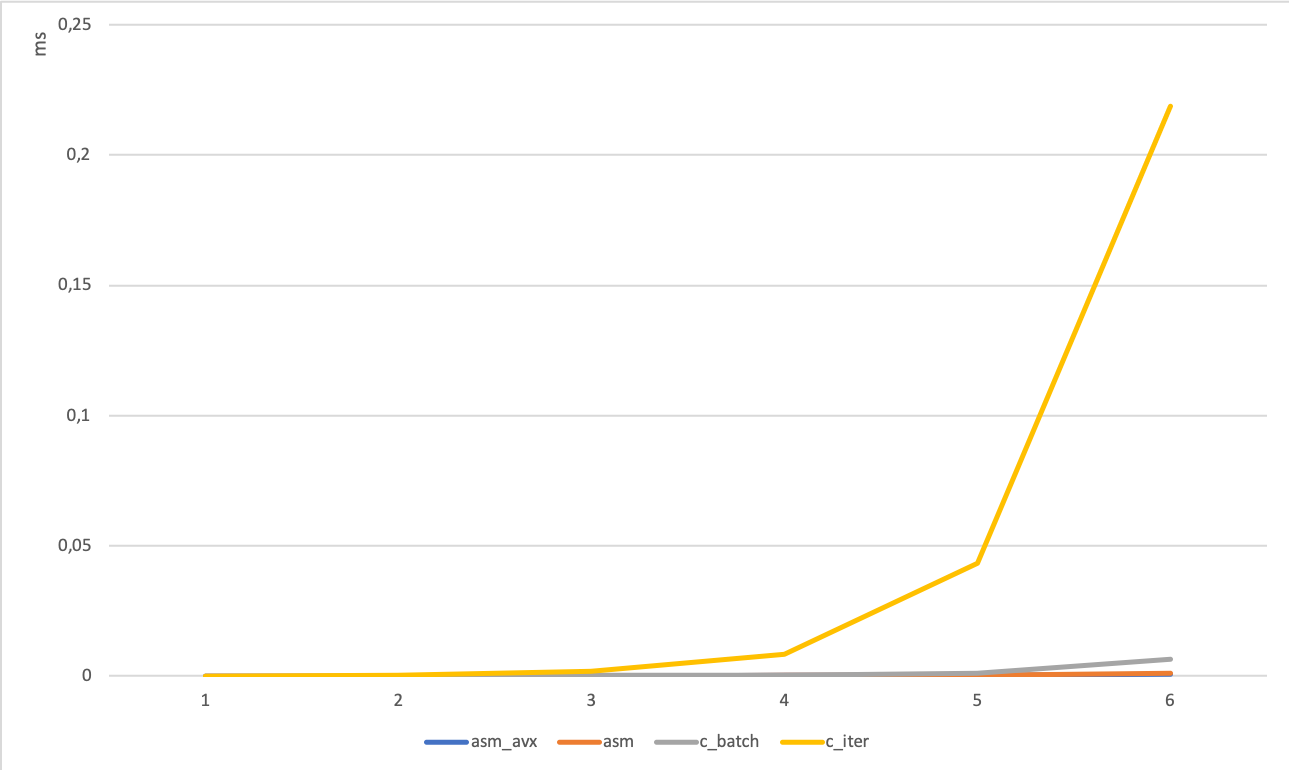
\includegraphics[width=0.45\textwidth]{laufzeitvergleich_1-6_alle_impl.png} }}%
    \qquad
    \subfloat[ohne \textit{c\_iter}]{{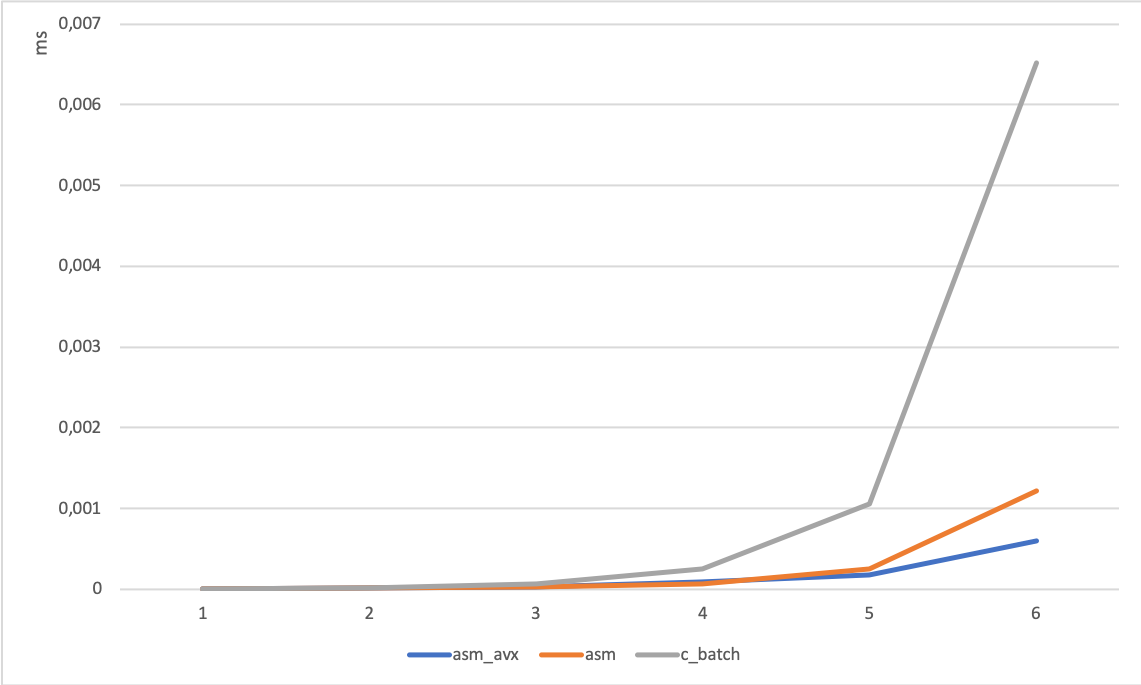
\includegraphics[width=0.45\textwidth]{laufzeitvergleich_1-6_fast.png} }}%
    \caption{Laufzeitverhalten der vier Implementierungen bis Grad 6}%
    \label{fig:Laufzeitvergleich}%
 \end{figure}
 
 \subsection{Iterative Berechnung der Moore-Koordinaten}
Aus Abb. 1 geht klar hervor, dass die iterative Berechnung der Moore-Koordinaten (wie in Sektion 2 beschrieben) deutlich ineffizienter ist als die anderen Implementierungen. Ein Vorteil dieser Variante ist zwar, dass sie nur sehr wenige Speicherzugriffe benötigt, da alle Berechnungen in den Registern durchgeführt werden können und nur das Endergebnis in den Speicher geschrieben wird. Durch das rein iterative Vorgehen kann dieser Algorithmus jedoch nicht sinnvoll auf Datenebene parallelisiert werden. Auch kann der dynamische Ansatz, von dem die übrigen Implementierungen profitieren, hier nicht angewandt werden. Im folgenden liegt daher der Fokus auf den restlichen Implementierungen.

\subsection{Vergleich Assembler- mit Referenzprogramm}
Die Implementierungen \textit{c\_ batch}, \textit{asm\_avx} und \textit{asm} ... siehe Section 3 ... \newline
An Abb. 1.b und den Benchmarkwerten kann man erkennen, dass die Assembler Implementierungen deutlich performanter sind als die C-Referenzimplementierung. Für Grad 6 ist die Assembler-Implementierung, welche 128-bit Register benutzt, drei mal schneller als das C-Programm. Dies ist darin begründet, dass sich die dynamische Berechnung der Hilberkurve optimal durch SIMD parallelisieren lässt. Somit können einige Koordinaten gleichzeitig innerhalb einer Operation verarbeitet werden. Die Anzahl der Punkte, die in ein SIMD-Register passen ist abhängig vom Datentypen der Koodinaten und der Größe der Vektorregister. Wir haben uns entschieden, von der in der Aufgabenstellung vorgegebenen Signatur \texttt{moore(uint64\_t degree, uint64\_t *x, uint64\_t *y)} abzuweichen und 32 bit Integer zu benutzen. Der maximale darstellbare Wert verringert sich dadurch zwar auf $2^{32}-1$, jedoch werden größere Werte erst ab einem $n > 32$ benötigt. Der Speicherbedarf einer Moore Kurve mit Grad 33 betrüge $4^{33} \cdot 2 \cdot 4 \text{ Bytes } \approx 590 \cdot 10^{18} \text{ Bytes}$, wenn man alle Koordinaten als 32 bit unsigned Integers darstellen könnte und das Doppelte bei Benutzung von 64 bit Integern. 
\newline
Durch die Reduzierung auf 32 bit Intger können nun bei Verwenung von 128 bit Vektorregistern vier und bei 258 bit Registern acht Werte gleichzeitig verarbeitet werden (siehe Abb. 2).

\begin{figure}[htbp] 
    \centering
    \subfloat{{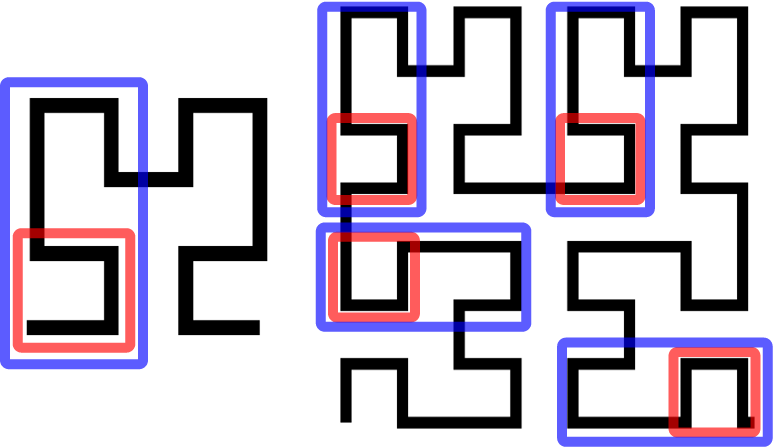
\includegraphics[width=0.69\textwidth]{hilbert_transformation.png} }}%
    \caption{Parallelisierung durch SIMD}%
    \label{fig:SIMD}%
\end{figure}

Durch Disassemblieren der mit \texttt{-march=native -O3} kompilierten Binärdatei festgestellt haben, dass der Compiler den C Code nicht vektorisiert. Daher war unsere anfängliche Vermutung, dass \textit{asm\_128} etwa vier mal so schnell ist wie unsere C-Implementierung und \textit{asm\_256} in der Hälfte der Zeit von \textit{asm\_128} terminiert.

\begin{figure}[htbp] 
    \centering
    \subfloat[Speedup Assembler- ggü. C-Implementierung]{{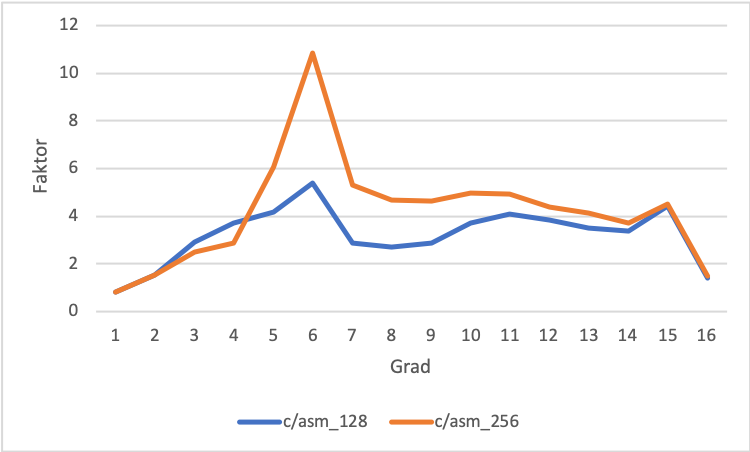
\includegraphics[width=0.45\textwidth]{speedup_base_c.png} }}%
    \qquad
    \subfloat[Speedup \textit{asm\_256} ggü. \textit{asm\_128}]{{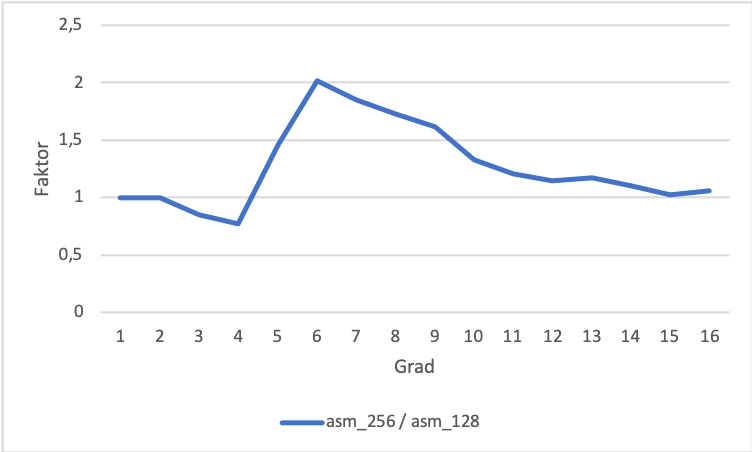
\includegraphics[width=0.45\textwidth]{speedup_base_asm_128.png} }}%
    \caption{Laufzeitvergleich C/ASM}%
    \label{fig:Laufzeitvergleich}%
 \end{figure}
 
 Abb. 3.a bestätigt den ersten Teil unserer Vermutung. Zwischen Grad 4 und 15 ist die \textit{asm\_128} Implementierung 2,8 bis 5,3 mal schneller als die Referenzimplementierung in C. Der zweite Teil trifft nur teilweise zu. Wie in Abb. 3.b zu sehen ist, profitieren vor allem Grade zwischen 6 und 10 von den größeren Vektorregistern. Bei größeren Graden bietet die Verwendung von AVX-Registern keine signifikante Performanzsteigerung.
 
\subsection{Cache Effizienz}
Abb 3.a wirft die Frage auf, weshalb die Assembler Implementierug bei Grad 6 besonders performant ist. Dies lässt sich vermutlich damit beantworten, dass die Moore Kurve sechsten Grades genau \textit{32 KiB} an Speicher benötigt und die Größe des L1 Caches der Maschine auf der getestet wurde \textit{32 KiB} beträgt. Um diese Annahme zu überprüfen wurde das Programm mit dem MacOS Tool \textit{Instruments} auf Cache-Misses (insbesondere L1) überprüft, mit dem Ergebnis, dass 6 der höchste Grad ist, bei dem noch nahezu keine L1 Misses auftreten.

\begin{figure}[htbp] 
    \centering
    \subfloat[Grad 1 - 15]{{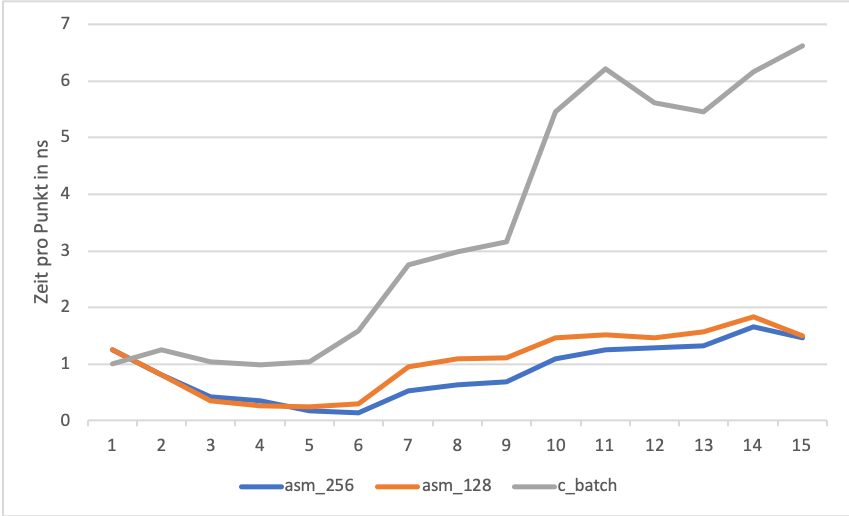
\includegraphics[width=0.45\textwidth]{ns_per_coord_1-15.png} }}%
    \qquad
    \subfloat[Grad 1 - 16]{{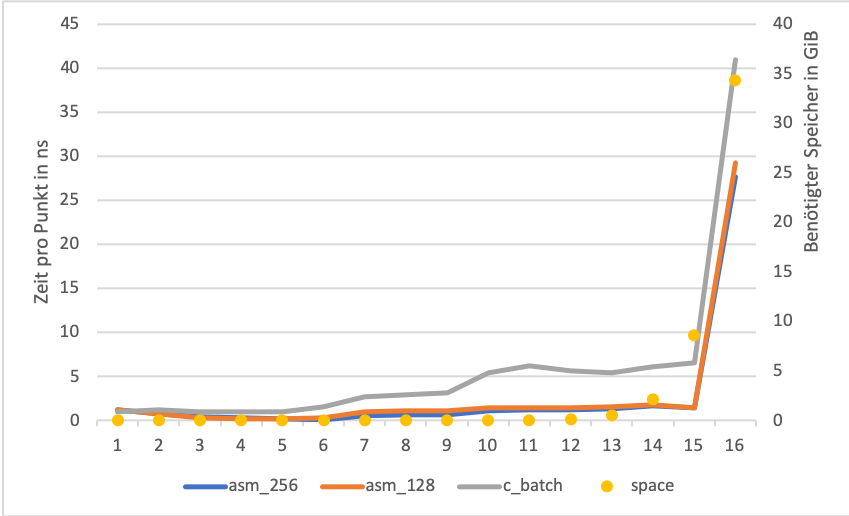
\includegraphics[width=0.45\textwidth]{ns_per_coord_1-16.png} }}%
    \caption{Nanosekunden pro Punkt der Moore Kurve}%
    \label{fig:Laufzeitvergleich Skaliert}%
 \end{figure}
 
 Der Vollständigkeit halber muss noch der Effizienzeinbruch bei Grad 16 angesprochen werden. Dieser ist damit zu erklären, dass die Speicheranforderung für die Berechnung der Moore Kurve auf 32GiB steigt. Da unser Computer nur 16 GiB an Arbeitsspeicher zur Verfügung stellt, müssen nun häufig Speicherseiten auf die Festplatte ausgelagert werden, was zu starken Performanzeinbußen führt.


\section{Zusammenfassung und Ausblick}

% TODO: Fuegen Sie Ihre Quellen der Datei Ausarbeitung.bib hinzu
% Referenzieren Sie diese dann mit \cite{}.
% Beispiel: CR2 ist ein Register der x86-Architektur~\cite{intel2017man}.
\bibliographystyle{plain}
\bibliography{Ausarbeitung}{}

\end{document}
